\documentclass[12pt, a4paper]{article}

\usepackage[frenchb]{babel}
\usepackage[T1]{fontenc}
\usepackage[left=2.2cm, right=2.2cm, top=2.5cm, bottom=2.5cm]{geometry} % Mise en page
\usepackage{tikz}
\usepackage{lscape}
\usepackage{graphicx}

\author{Florian \bsc{Thuin} (06561100) \and Gregory \bsc{Vander Schueren}}
\title{LINGI1131 - Oz Project Report}
\date{\today}

\begin{document}

\maketitle
\section{Component diagram}

Our project is separated in many \og{}components\fg{} :

\begin{description}
 \item[Game] module : It's run when you start the program, it launches the intro to ask you to type a name and to choose a pokemoz if you don't autoplay. It initializes the game and then it loops until you go to the finish square.
 
 \item[GameIntro] : An interface which allows you to choose a name and a pokemoz to begin the game !
 \item[Fight] module : Manage the fight between trainers or trainer VS wild pokemoz.
 \item[AutoPilot] module : Manage the autoplay if this option is given in command line.
 \item[Map] : Design the map you see while playing.
 \item[Interface] : Design the part above the main interface where you see the fight, click for fight or run, etc.

\end{description}

\bigskip

Those components rely on \og{}helpers\fg{} :

\begin{description}
 \item[GameState] module : maintains the game\_state structure up-to-date with the game.
 \item[Player] module : maintains the player structure up-to-date with the game.
 \item[Pokemoz] module : maintains the pokemoz's structure up-to-date with the game.
 \item[Lib] module : do many things like get the arguments, write messages on console, create random numbers,...
 \item[Characters] module : contains every pokemoz's and trainers of the game.
 \item[CompileImages] : the image library (it's a QTk image library)
 
\end{description}

\begin{landscape}

\begin{figure}

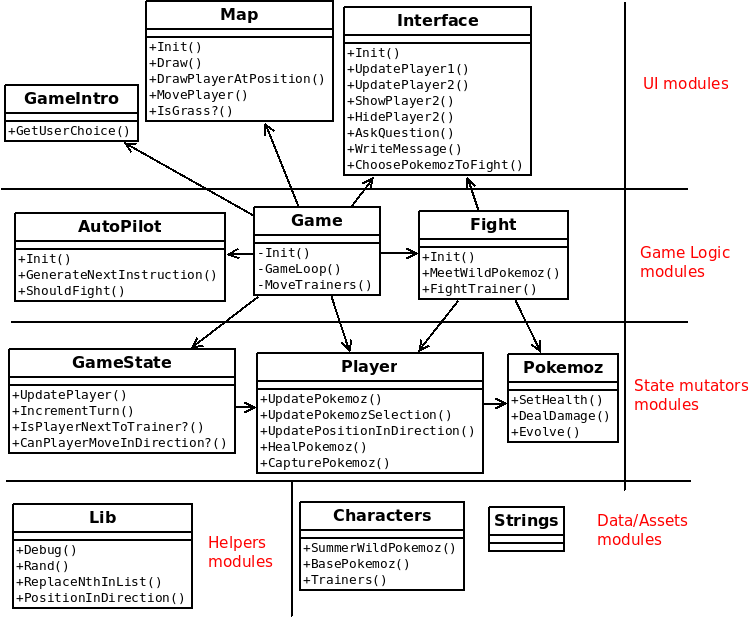
\includegraphics[width=\linewidth]{Diagramme1.png}
\caption{Component diagram of our project}
\end{figure}

\end{landscape}


\section{State diagrams}

\begin{figure}
 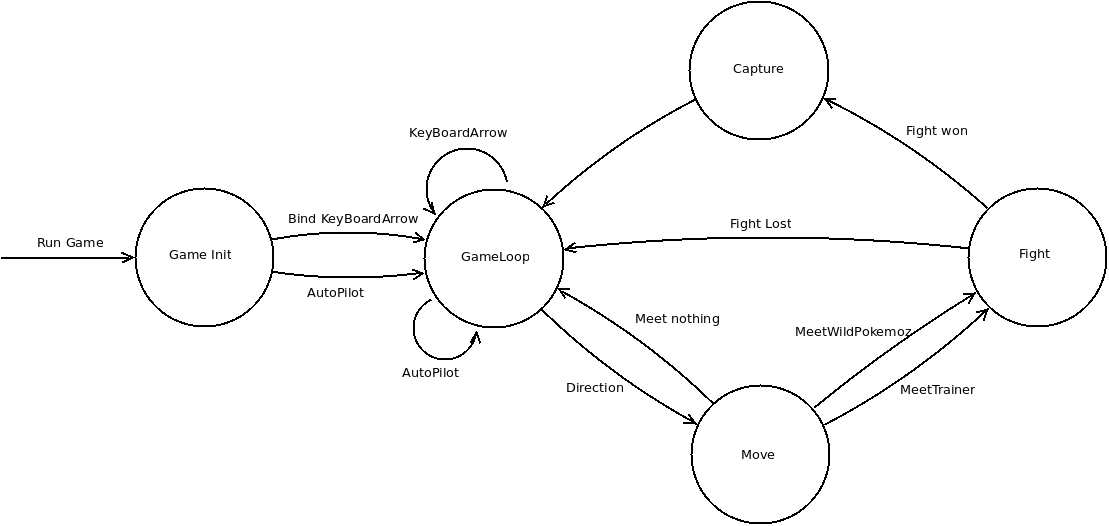
\includegraphics[width=\linewidth]{State_diagram_oz.png}
 \caption{State diagram of our project}
\end{figure}


\section{Discussion of data structures}

As it is described above, we have many \og{}modules\fg{}, which are in fact \textbf{functors}. These functors exchange mainly the \textbf{GameState}, which is a record that contains almost everything.
It contains : the number of instructions received, a player record and a list trainers record. The player record contains all informations about the state of the player (the pokemoz he has, the position where he is,...). 
It's the same kind of information that a trainer record stores. 
That's why exchanging GameState is sufficient for almost all methods that needs to know something about the game. However, using such a complete structure to discuss between modules has a drawback : it may be more complex to understand the \og{}little methods\fg{}, but it simplifies so much the big ones and the calls of procedures that it is worth.



\end{document}